% @author Marcel Ruland (2018)
%
% Random pieces of information I picked up along the way (might turn out useful):
% [chapterprefix=true] changes ``1 LaTeX'' to ``Chapter 1\\ LaTeX''

%% tell TeXshop to compile using LuaLaTeX and encode with UTF-8
%!TEX TS-program = lualatex
%!TEX encoding = UTF-8 Unicode

\documentclass[DIV=calc,BCOR=0mm,pagesize,toc=bib,abstract=true]{scrreprt}
% [toc=bib] includes bib in toc
% [abstract=true] displays abstract title
\usepackage{../sty/ba_style}  % loading packages, typesetting, etc.


% using all commands now to have an exhaustive list and see what they're all doing, will probably remove some of them at some stage
\titlehead{Titlehead, whatever\ldots}
\subject{Universität Paderborn}
\title{Applying Frequent Pattern Mining to Multimodal Behaviour in Interaction}
\subtitle{Visualising Significant Patterns}
\author{Marcel Ruland\thanks{Oh deer how thankful am I\ldots}}
\publishers{Publishing Publishers}
\dedication{Totally dedicating this to me, myself, and I, because no one even knows this thing exists.}

\begin{document}
\maketitle
%% @author Marcel Ruland (2018)

\begin{abstract}
Human social interaction can be characterised by multimodal behaviour. According to theoretical positions emphasising that communication is organised by the interaction partners jointly, we identified the challenge of assessing human sequential behaviour that is spread across different modalities and co-constructed with a partner. In previous work, we faced the challenge by applying frequent pattern mining in an analysis of a corpus of mother-child dyads.

The application of frequent pattern mining provided some support and initial results for the proposition that human interactive behaviour is sequentially organised. Accordingly, verbal and nonverbal behaviour are co-constructed by the interaction partners and form a range of patterns. For example, with respect to the occurrence of maternal vocal behaviour, some nonverbal framing was notable. Firstly, one pattern with a high confidence suggests an intrapersonal sequence of gazing at the infant, smiling, and speaking. In contrast, another pattern suggests an interpersonal sequence of mother gazing at her infant, infant gazing back followed by vocal behaviour of the mother. The analysis reveals patterns emerging between infants as young as 3-months-old and their mothers.

Taken together, frequent pattern mining is a more exploratory analysis as the premises and conclusions emerge as a result of it. While this method yields contingencies and dependencies and provides their frequencies, it is not yet investigated how the significance of these patterns can be calculated and how it can be visualised. Our paper presents first solutions to the problem of how to discern and visualise the significance of some patterns with respect to other existing patterns in the sample.
\end{abstract}
\tableofcontents

% !TEX root = ../ba_master.tex
% @author Marcel Ruland (2018)

\chapter{Introduction}
A \emph{turn} is a basic unit of speech in conversation. When a speaker begins their turn, they gain the right to speak and\dash upon finishing their utterance\dash pass that right to another participant of the conversation. A turn is on average 2~sec.\ in length with very high variation. They usually consist of syntactically complete clauses and give pragmatically sufficient information, though this is by no means a necessity \citep[\pnum{8}]{levinson16}. \emph{Turn-taking} is the act of one speaker finishing their turn and another speaker beginning their turn, i.e.\ passing on the right to speak from one speaker to another.

\section{Previous Research}
\citep{levinson16} transition between speakers is three times faster than language encoding, psycholinguistics has studied language production and comprehension separately
%turn taking has so far been considered unimodal, until \citet{rohlfing18} came along
%brief explanation \fpm, there is only one single study so far

\subsection{Turn-Taking}

\subsection{\fpm}



\section{The Aim of this Study}
The present study builds on work by \citet{rohlfing18}, who applied \fpm{} techniques to a corpus of mother-child dyads, thereby identifying turn-taking as a multimodal phenomenon. It aims to further improve and operationalise this methodology for behavioural studies of similar sort.
introduce notion of significance, visualise significant patterns


























%\section{Pattern Mining Compared to Traditional Statistics}
%Statistical methods can broadly be divided into two subgroups. \emph{Inferential statistics} is concerned with methods suited to affirm or reject a given hypothesis in a data set, where the hypothesis is formulated in advance. A canonical example are significance tests, where we formulate a null-hypothesis and then perform tests to determine whether it can be affirmed\footnote{``affirmed'' in the sense of ``not proven, but no evidence against it either''} or rejected. \emph{Exploratory statistics} on the other hand do create new hypotheses. With no hypothesis formulated in advance, the tests are performed on a data set and the results may be used to formulate new hypotheses afterwards. A canonical example hereof is the relatively young field of \fpm.
% @author Marcel Ruland (2018)

\chapter{Applying Frequent Pattern Mining}
\section{Method}
The following subsections begin by introducing the raw data \emph{as-is} and then proceed by describing the process of annotating and evaluation the data, thus going steadily from concrete to more and more abstract representations. I begin by describing the content of the video corpus and end with abstract rules\footnote{For the definition of \emph{rule} here, see section \ref{sec:mining} on page~\pageref{sec:mining}.}.

\subsection{The Nature of the Data}
Explain what happens in the videos basically, not yet talking about coding the data.

\subsection{Annotation of the Videos}
11 kinds of events were hand-coded for both mother and child using the \textsc{elan} software \cite{wittenburg06}. These categories were of linguistic, vocal, and visual modality. Categories were chosen HOW??  % ELABORATE here
Table \ref{tab:categories} lists all categories. Every annotation contains a start and end time point and therefore also the duration of the respective event. This way, sequences as shown in Figure \ref{fig:idealseq} are obtained (note that this is a fictional sequence). \fpmlabel{A}, \fpmlabel{B}, and \fpmlabel{C} are three different kinds of events; the x-axis represents time. We see two occurrences of type \fpmlabel{A} and \fpmlabel{B} each, as well as a longer occurrence of type \fpmlabel{C}. Those time points that are indicated on the x-axis mark the beginning and/or end time point of a specific occurrence. All occurrences of a dyad together are referred to as a sequence, i.e.~there are 11 sequences in the corpus.

% @author Marcel Ruland
\begin{table}
\center
	\begin{tabular}{>{\ttfamily}ll} 
	\toprule
	{\rmfamily Category}			& Explanation \\
	\cmidrule(lr){1-1} \cmidrule(lr){2-2}
    mother-speech					& explanation goes here \\
	m-voc							& explanation goes here \\
	m\_gaze\_at						& explanation goes here \\
	m\_gaze\_away					& explanation goes here \\
	m\_gaze\_at\_object				& explanation goes here \\
	mo\_smile						& explanation goes here \\
	\cmidrule(lr){1-1} \cmidrule(lr){2-2}
	infant\_vocalizations\_infant	& explanation goes here \\
	i\_gaze\_at						& explanation goes here \\
	i\_gaze\_away					& explanation goes here \\
	i\_gaze\_at\_object				& explanation goes here \\
	inf\_smile						& explanation goes here \\
	\bottomrule
	\end{tabular}
	\label{tab:categories}
	\caption{Categories coded in the data}
\end{table}
% @author Marcel Ruland (2018)
\begin{figure}
{\sffamily\addfontfeature{Numbers=Lining,Letters=Uppercase}
	\center
	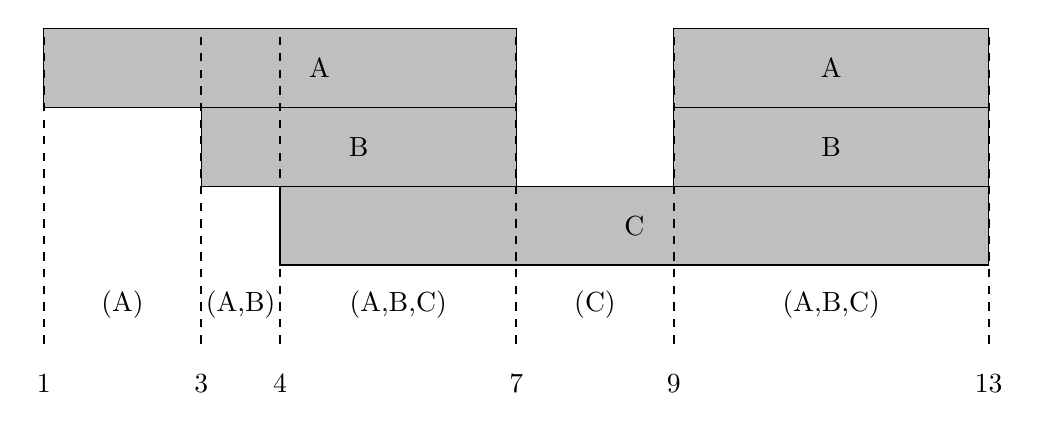
\begin{tikzpicture}
%		\draw [help lines, dashed] (0,0) grid (12,5);  % help lines
		
		% boxes
		\draw [fill=lightgray] (0,4) rectangle (6,5);  % A1
		\node at (3.5,4.5) {A};
		
		\draw [fill=lightgray] (8,4) rectangle (12,5);  % A2
		\node at (10,4.5) {A};
		
		\draw [fill=lightgray] (2,3) rectangle (6,4);  % B1
		\node at (4,3.5) {B};
		
		\draw [fill=lightgray] (8,3) rectangle (12,4);  % B2
		\node at (10,3.5) {B};
		
		\draw [fill=lightgray] (3,2) rectangle (12,3);  % C
		\node at (7.5,2.5) {C};
		
		% item sets
		\node at (1,1.5) {(A)};
		\node at (2.5,1.5) {(A,B)};
		\node at (4.5,1.5) {(A,B,C)};
		\node at (7,1.5) {(C)};
		\node at (10,1.5) {(A,B,C)};
		
		% time points
		\node at (0,0.5) {1};
		\node at (2,0.5) {3};
		\node at (3,0.5) {4};
		\node at (6,0.5) {7};
		\node at (8,0.5) {9};
		\node at (12,0.5) {13};
		
		% time point lines
		\draw [dashed, thick] (0,1) -- (0,5);
		\draw [dashed, thick] (2,1) -- (2,5);
		\draw [dashed, thick] (3,1) -- (3,5);
		\draw [dashed, thick] (6,1) -- (6,5);
		\draw [dashed, thick] (8,1) -- (8,5);
		\draw [dashed, thick] (12,1) -- (12,5);
		
		% text representation
	%	\node at (6,0) {\code{<(A [1,3]),(A,B [3,4]),(A,B,C [4,7]),(C [7,9])(A,B,C [9,13])>}};
	\end{tikzpicture}
	\caption{Graphical representation of an idealised sequence}
	\label{fig:idealseq}
}
\end{figure}

\subsection{Mining Approach}
\label{sec:mining}
The fundamental aim of \fpm~techniques is to find patterns in a data set that occur \emph{frequently}. The specific kind of pattern and the definition of \emph{frequent} cannot be generalised and depend heavily on the individual application. In contrast to descriptive and inferential statistics, which disprove or affirm hypotheses generated beforehand, \fpm~is of an exploratory, hypothesis-generating nature. Depending on the patterns found, one may then formulate hypotheses afterwards, which may then in turn be tested empirically using descriptive and inferential statistics \cite[6~ff.,~tba]{rohlfing18,han12}.%% ISSUE: How do you give page references for each individual source when citing multiple sources?

\subsubsection{Association Rules}
The patterns \citeasnoun{rohlfing18} looked for were association rules of the form \fpmrule{A}{B}, where the probability of the succedent \fpmset{B} was high given the antecedent \fpmset{A}. Note that antecedent and succedent are not single events but sets of events. One may equally well form a hypothetical rule of the form \fpmrule{B,D}{A,C,D}. Occurrences of a rule were taken into account if they fulfilled one of two conditions:

\begin{enumerate}
	\item The antecedent's start time point lies before that of the succedent.
	\item The antecedent's and succedent's start time points are identical, i.e.~they begin simultaneously.
\end{enumerate}

Referring again to Figure \ref{fig:idealseq}, one can for example observe the rules \fpmrule{A}{B} and \fpmrule{A}{B, C} (because the start time point of the antecedent lies before that of the succedent), but not \fpmrule{B}{A}.


\section{Results}

%\subsection{Association Rules}
%In the following, I will first lay out the type of association rule used by \citeasnoun{rohlfing18} and then explain how I modified this scheme to better fit the interactional, multimodal nature of the data. The basic sequence is structured as follows:
%\begin{quote}
%	\code{<(A [1,3]),(A,B [3,4]),(A,B,C [4,7]),(C [7,8]),(A,C [8,9]),(A,B,C [9,13])>}
%\end{quote}
%
%In traditional sequential pattern mining, the basic data type---called a sequence---is an ordered set of (unordered) item sets \cite[p.~588~ff.]{han12}. Here, every item set in the sequence has an additional annotation marking the start and end time points between which the item set (that is, one specific occurrence of it) is contained in the data. Figure \ref{fig:idealseq} gives a graphical representation of this example sequence. Rules of the sort \fpmrule{A}{B} must fulfil one of two conditions:
%\begin{enumerate}
%	\item The antecedent's start time point lies before that of the succedent.
%	\item The antecedent's and succedent's start time points are identical, i.e.~they begin simultaneously.
%\end{enumerate}
%Therefore, in the example sequence one can observe the rules \fpmrule{A}{A,B} but not \fpmrule{B}{A,B}. The following three modifications improve the scheme to better fit the data:
%
%\paragraph{Imprecision of hand-coded data}
%The second condition is problematic given the nature of the data. Every annotation has been hand-coded and with coding by hand comes imprecision. Given the fact that the time points' are precise up to one millisecond, there will in all likelihood not be any two annotations that begin at the exact same point. After examination of the source files (i.e.~\textsc{elan} files) and consultation with the coders I have decided to allow for a \imprecisiondelay~delay such that two annotations \(a\) and \(b\) are treated as beginning simultaneously iff their start time points \(s_a\) and \(s_b\) lie no further than 300ms apart (\(|s_a - s_b| < 300ms\)). This delay accounts for the coders' imprecision.
%
%\paragraph{Inter- and intrapersonal rules}
%Given the dyadic nature of the data it is necessary to distinguish between inter- and intrapersonal rules not only in rule evaluation but already in the mining process. Depending on various factors, the average human reaction time to an event lies between XXX and XXXms. %values? source?
%It follows that if both mother and child begin an event at the same time or with a delay below reaction time, then the cooccurrence is pure chance and should not be considered a pattern. Analogous to the maximum delay described in the previous paragraph, interpersonal sequences are only considered with a minimum delay of \reactiontime~between the time start points.



%zero delay only in intrapersonal rules, minimum delay for interpersonal rules -- reaction time

























% @author Marcel Ruland (2018)

\chapter{Establishing a Notion of Significance}
\section{Method}
create null distribution by shuffling relative positions of events, then test for significance using tests suited for skewed distribution

Tests to be used:
- some sort of significance test
- support(X->Y) = P(XUY) and confidence(X->Y) = P(Y|X), both associated with an \emph{arbitrary} cutoff threshold \cite[p.~21~ff.]{han12}

``[M]any patterns that are interesting by objective standards may represent common sense and, therefore, are actually uninteresting.'' \cite[p.~22]{han12}
\section{Results}
show and discuss significant rules
% @author Marcel Ruland (2018)

\chapter{Visualising Significant Patterns}
\section{Identifying the Challenge}
Which questions should be answered in an instant? Which information is vital, which information is neglectable and why?

\section{Ways of Evaluating Visualisations}
several metrics from Cairo's books

\section{Proposing a Visualisation} % so so so much a working title omg I can't even
this is where the actual visualisation is introduced and explained

%\appendix
%% @author Marcel Ruland (2018)

\chapter{Appendix}
\lipsum

%\listoftables
%\listoffigures
\bibliography{../bib/ba_bib}

\end{document}
